\section{Background}
  In this section I will discuss the background work and research done for this project. I will start by disusing my teams place in the organisation and 
  our OKRs, explaining how this project helps us hit these objectives. I will then outline the current architecture and the initial design for the project.
  Finally I will discuss some areas of interest around project, these include cloud computing, database parallelisation strategies and CI/CD challenges.

  \subsection{Organisation and Team}
  The BBC is broken into multiple layers with different responsibilities and goals. I am in a team called \textit{SpaceChimps} which is part of
  the partnerships group, which itself is in the product group.

  \begin{figure}[H]
    \centering
    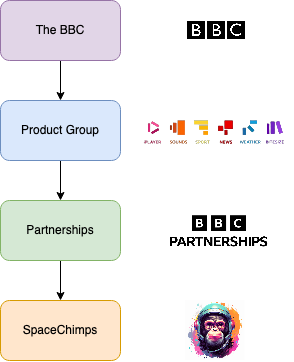
\includegraphics[width=4cm]{assets/bbcHierarchy.drawio.png}
    \caption{Image showing SpaceChimps place in the BBC (Bowker, 2023).}
    \label{fig:bbcHierarchy}
  \end{figure}

  Our main aim as a team is to provide data to partners that they can use on their devices to promote BBC content. The project described in this report does
  just that by providing schedules for live content to partners. This aim fits directly into Partnerships objectives:

  \begin{itemize}
    \item The main objective of the schedules pipeline was to deprecate a service called \textit{nitro}. This is an external platform the BBC 
    used to distribute some of its data to partners. However this was a costly solution and meant we didn't have full control over the process. 
    This projects aim is to improve this system allowing us to have better metrics and control over the data we share, providing the most up to
    date and relevant schedules.
    \item It helps drive growth as we are able to get content out to more people on more devices, increasing exposure to the BBC.
    \item It helps us improve our partner experience by working with them on integrating the data into their feeds.
    \item This project reduces the total time processing data, which therefore reduces our costs and makes us more sustainable.
  \end{itemize}

  \footnote{\textbf{B1} - This shows how the project accomplishes organisational goals.}
  All objectives can can be seen in \hyperref[sec:AppendixA]{\textbf{Appendix A}} (BBC Partnerships, 2023).

  As well as schedules we also provide a \textit{'catalogue'} of episodes, series and brands that are currently available on iPlayer.

  \begin{figure}[H]
    \centering
    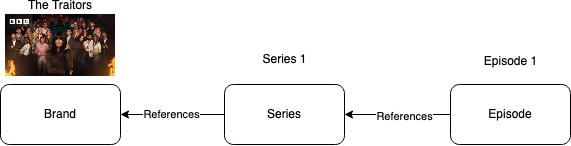
\includegraphics[width=10cm]{assets/catalogueHierarchy.drawio.png}
    \caption{Image showing catalogue hierarchy and how they reference each other.}
    \label{fig:catalogueHierarchy}
  \end{figure}
  
  We provide both a 0 day and 8 day catalogue, these containing programme data that are available now or up to 8 days in the future. We 
  also have an \textit{'unfiltered'} catalogue that is not available to partners which contains all programme data with no availability limits.
  This unfiltered catalogue is what is used by the schedule pipeline to get it's data about episode/series/brands within the schedule.

  \subsection{Original Architecture}
  The original solution was composed of AWS services that created a pipe and filter architecture which transformed inputs into multiple outputs 
  (Somerville, 2016, pp.182-183) that can be used by partners. The figure below shows this architecture.
  
  \begin{figure}[H]
    \centering
    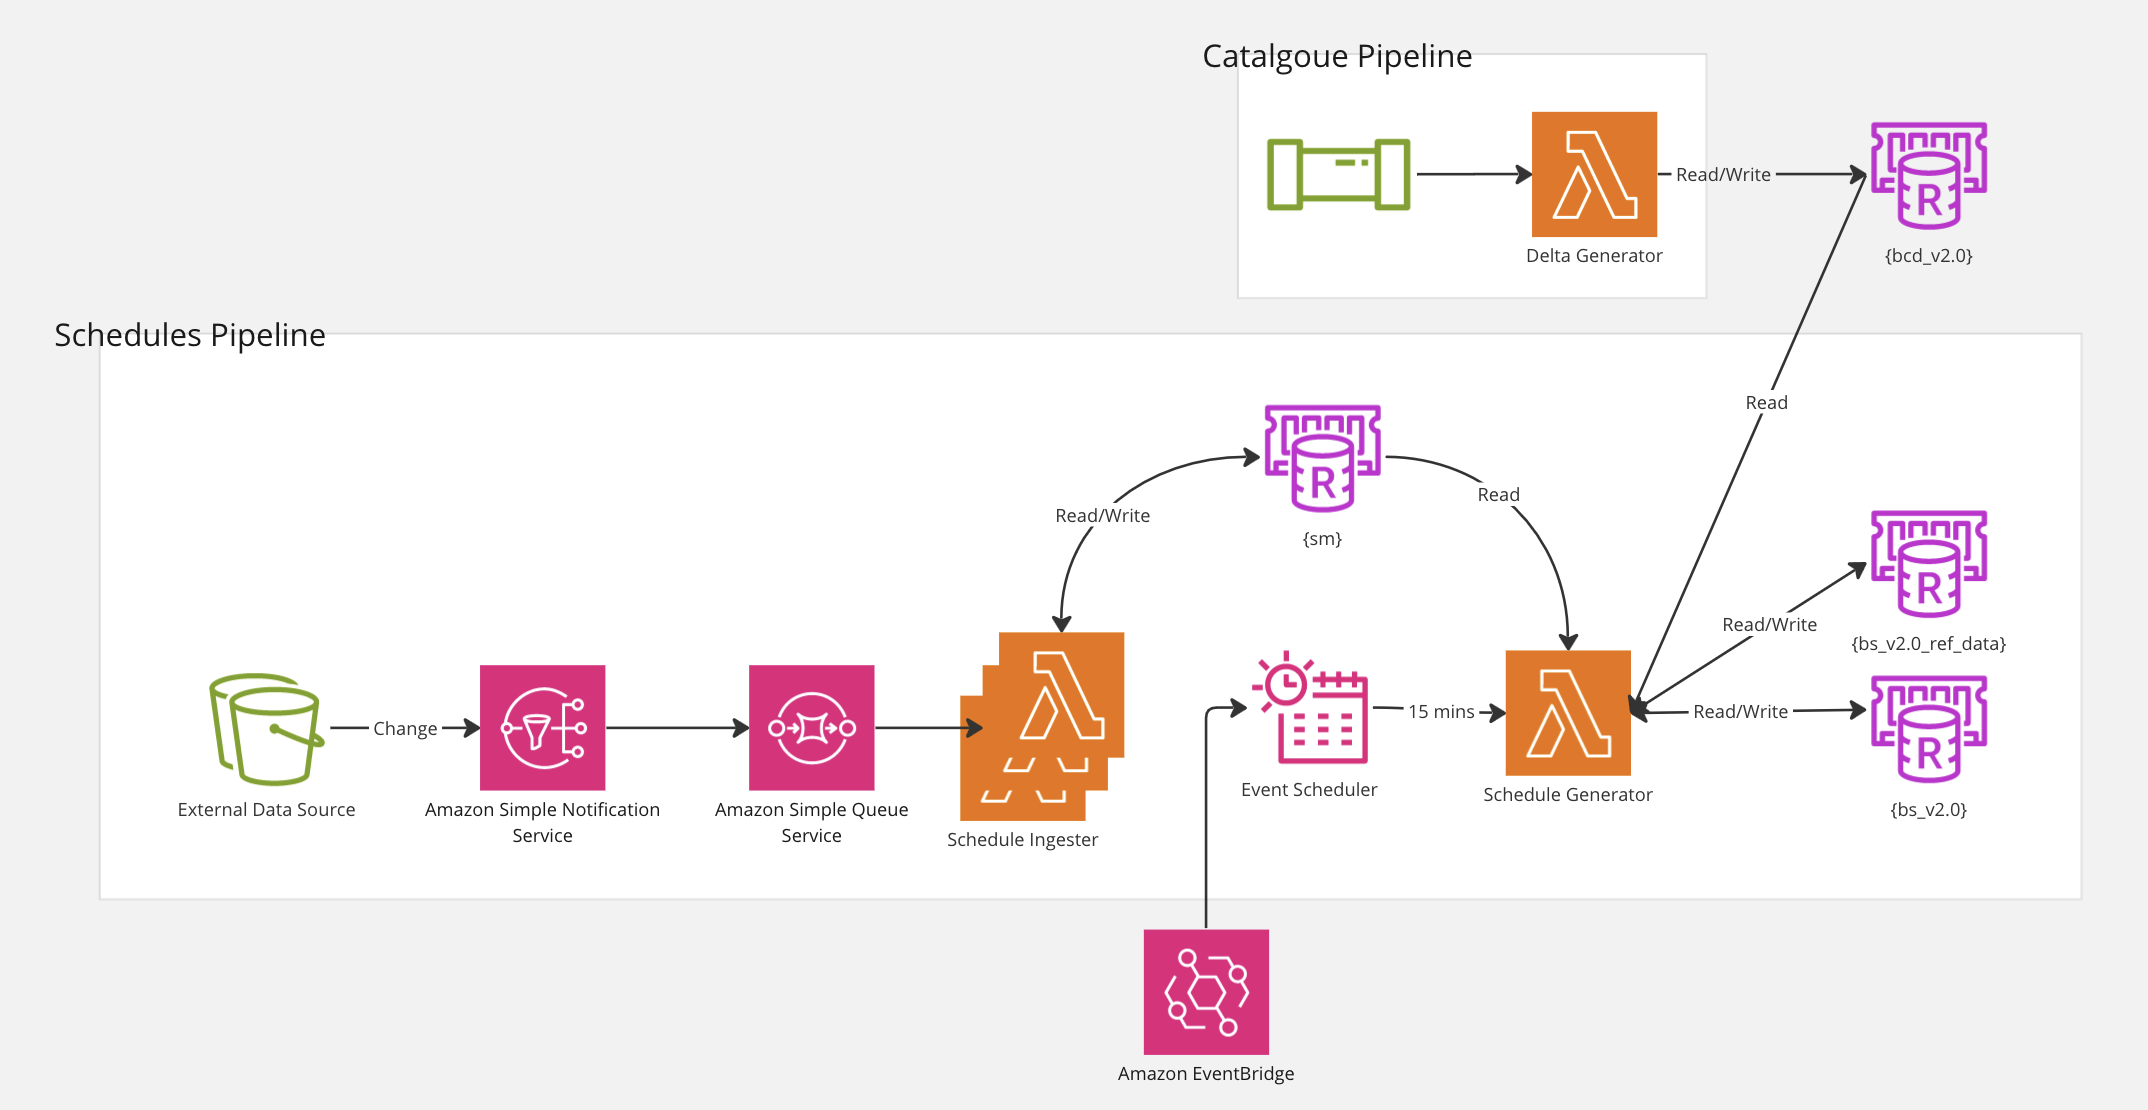
\includegraphics[width=12cm]{assets/architectures/starting.png}
    \caption{Image showing the initial architecture.}
    \label{fig:initialArchitecture}
  \end{figure}

  A pipe and filter architecture is achieved with the combination of AWS lambda (Amazon Web Services, 2024a) with updates being triggered by a publish/subscribe 
  model (Somerville, 2021, p.179) achieved through AWS' Simple Notification Service (SNS) (Amazon Web Services, 2024b) and Simple Queue Service (SQS) 
  (Amazon Web Services, 2024c) with the former publishing and the latter subscribing. The lambda only runs when a message is published to the SQS, this triggers 
  the lambda and the pipeline begins precessing the new message.

  The data is updated by an external system in AWS S3 (Amazon Web Services, 2024d), this publishes a message that the data has changed, our first lambda 
  (the ingester) receives this message and processes/stores it into a \textit{'common'} model that's used internally only. Our internal model is then up to date,
  however our partner facing model, created by the schedule generator, is not. In the original system this lambda was not driven by events, but instead ran every
  15 minutes and processed all the schedules in one go, whether they had updated or not. 
  
  \begin{figure}[H]
    \centering
    \includegraphics[width=10cm]{diagrams/activity/Old Coldstart.png}
    \caption{Activity diagram showing schedule generators logic.}
    \label{fig:oldColdstart}
  \end{figure}

  This could leave partners with data up to 15 minutes out of date, dependant on when they retrieve the data, resulting in end users being shown incorrect
  schedules. 

    \subsubsection{Initial design solution}
    \footnote{\textbf{SE-K02} - This initial design helped us do a spike which lead to the considerations for future work and immediate changes to this design.}
    The schedules pipeline also requires data from our catalogue pipeline, for titling, descriptions, viewer discretion warnings and subtitles. For this 
    reason it needs to be alerted when catalogue data changes as well as when schedules change. An initial design had already been complete before the work 
    started by another member of the team.

    \begin{figure}[H]
      \centering
      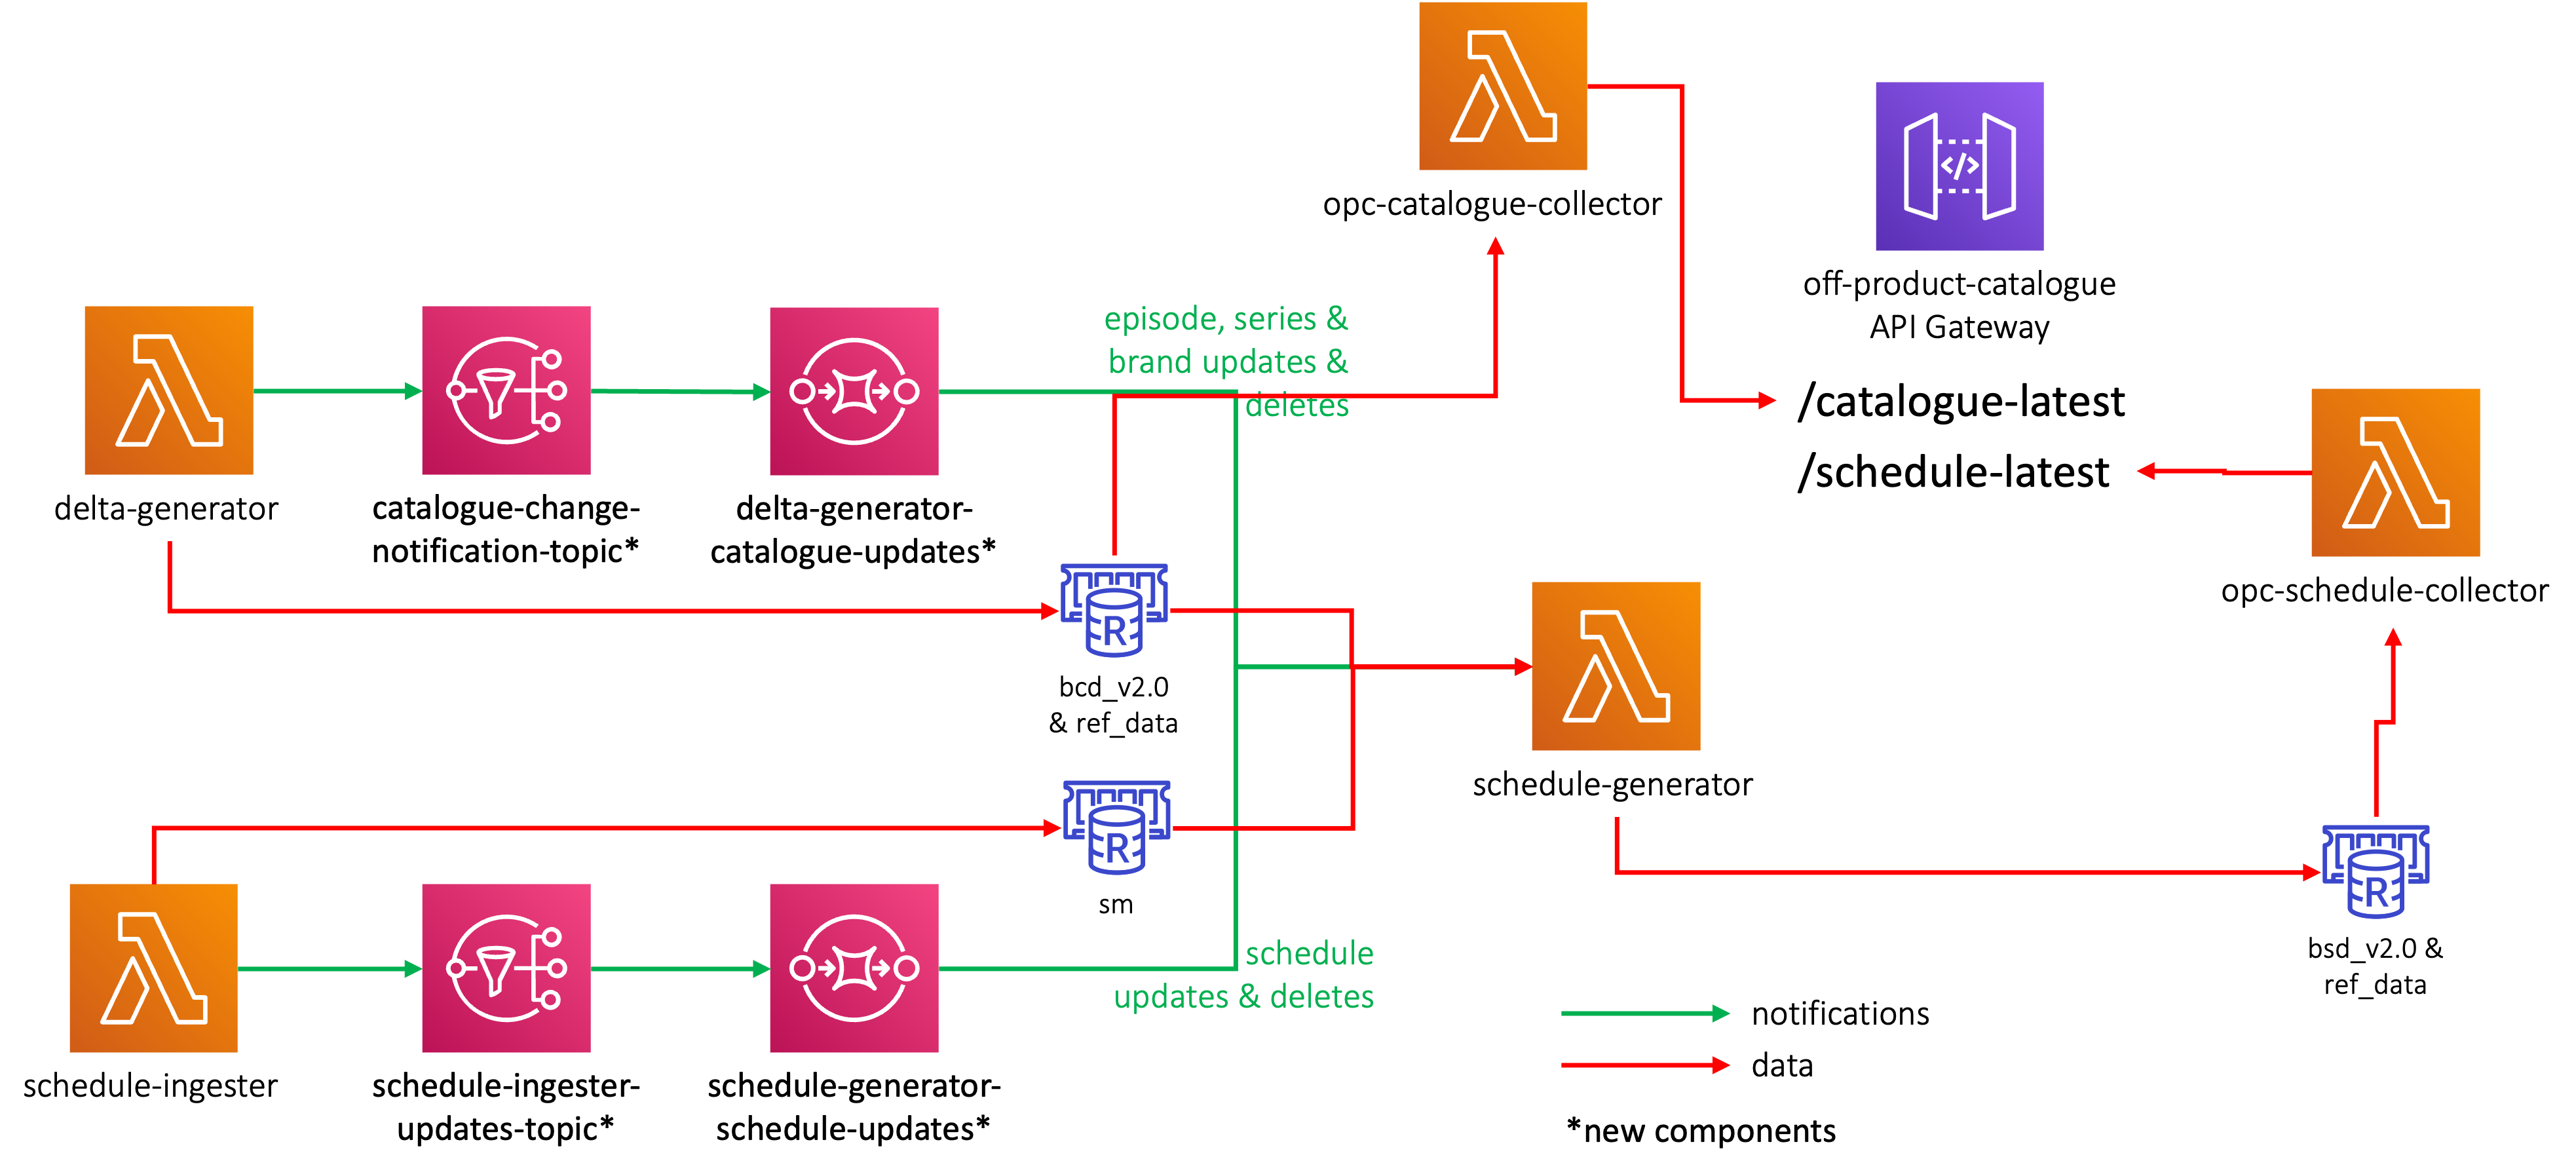
\includegraphics[width=12cm]{assets/initialDesign/architecture.png}
      \caption{Image showing the initial updated schedules design (Lloyd, 2023).}
      \label{fig:initialDesign}
    \end{figure}

    The above diagram has been edited down to include only work related to the project, a full diagram including notifications being directly sent to partners can 
    be found in \hyperref[sec:AppendixB]{\textbf{Appendix B}}. This diagram also includes our endpoints and collectors that partners use to 
    retrieve the data. This proposed system uses the pub/sub model described earlier and will subscribe to both catalogue and schedule events.

    Alongside the architectural design an algorithm was proposed for these events.
    \begin{itemize}
      \item \textbf{For schedule updates} - We want to update the partner facing model of the schedule linked in the notification. This schedule has a 
      list of broadcasts that map to episodes in the catalogue. A list should be maintained within each episode to create a link between both, allowing episode 
      updates to trigger updates to schedules that reference them. All catalogue data referenced in a schedule should be copied over to the schedules keyspace,
      leaving the catalogue keyspace and items untouched.
      \item \textbf{For schedule deletes} - Remove schedule from store, and remove schedule reference from list contained within each episode that schedules 
      references in its list of broadcasts.
      \item \textbf{For catalogue/programme updates:}
        \subitem \textbf{For episodes} - Update episode in store, update each schedule that is linked in episodes broadcast list.
        \subitem \textbf{For series/brands} - Get all episodes linked to either the series or brand, update each schedule that is linked in each episodes 
        broadcast list.
    \end{itemize}

    Flow diagrams can be found in \hyperref[sec:AppendixC]{\textbf{Appendix C}} (Lloyd, 2023).

    With the addition of schedules and broadcasts lists in episodes, our relations between types objects can now be described in the below ERD diagram.

    \begin{figure}[H]
      \centering
      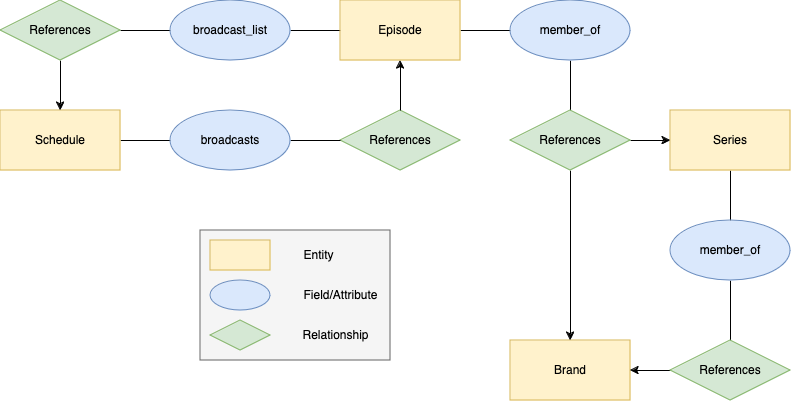
\includegraphics[width=8cm]{assets/dataERD.drawio.png}
      \caption{Relationships between types of data offered to partners.}
      \label{fig:relationshipsERD}
    \end{figure}

    Episodes and schedules will now link to each other via their associated fields.

\newpage
